\chapter{Secure Communication Protocol}

\begin{flushleft}
    \textcolor{red}{\textbf{\textit{Secure Communication Protocol at the Transport Layer}}} \\
    \textbf{\textit{Transport Layer Security}} e \textbf{\textit{Datagram TLS}} sono due protocolli che garantiscono sicurezza, rispettivamente, per i protocolli \textbf{TCP} e \textbf{UDP}.
    \begin{itemize}[nosep]
        \item il \textbf{TLS} è il protocollo maggiormente utilizzato per mettere in sicurezza le comunicazioni, con la sua ultima versione 1.3 sono state deprecate le versioni precedenti alla 1.2 (\textbf{TLS 1.1} e \textbf{1.2}) - le versioni deprecate possono essere utilizzate in sistemi \textit{legacy} ma devono essere configurate in maniera accurata per evitare o mitigare vulnerabilità note; precedentemente alla versione 1.0 il protocollo era chiamato \textbf{\textit{Secure Socket Layer - SSL}}.
    \end{itemize}
    \textbf{TLS} è, quindi, un protocollo di sicurezza che si posizione all'interno dello \textit{stack \textbf{TCP/IP}} tra il \textit{transport} e l'\textit{application layer} e viene utilizzato per i canali di comunicazione \textbf{\textit{stream oriented}}. 

    \smallskip

    Dopo la standardizzazione - nel 2018 - di \textbf{TLS 1.3} viene ancora considerata sicura la versione \textbf{1.2} ad eccezione per gli \textbf{schemi di crittografia deprecati}. Le versioni 1.1 e 1.0 sono deprecate dal \textit{web browser} dal 2020.

    \medskip

    \textbf{DTLS} è basato sul protocollo \textbf{TLS}, ma come \textbf{UDP} è \textbf{\textit{datagram oriented}}, in questo caso la versione 1.3 non è ancora standardizzata, ma ha come \textit{feature} la capacità di \textbf{\textit{replay detection}}. \\
    Per questioni di sicurezza \textbf{DTLS} necessita di un \textit{handshake} iniziale in modo da poter fare un \textit{key exchange} con la condivisione della chiave simmetrica di sessione, nel caso in cui essa fosse già precondivisa, l'\textit{handshake} viene rimosso.
\end{flushleft}

\newpage

\section{Transport Layer Security}

\begin{flushleft}
    Possiamo modellare il \textit{design} del protocollo indpendentemente dalla sua versione come due fasi:
    \begin{enumerate}[nosep]
        \item \textcolor{red}{\textbf{\textit{Handshake phase}}}: che a sua volta è divisa in:
        \begin{itemize}[nosep]
            \item \textbf{\textit{Negotation}}: server per definire le capacità (\textit{capabilities}) condivise tra client e server.
            \item \textbf{\textit{[Authenticated] Key Exchange}}: si va a deinire le chiavi che verranno utilizzate nella fase di trasporto - utilizza crittografia asimmetrica.
        \end{itemize}
        \item \textcolor{red}{\textbf{\textit{Transport phase}}}: vengono scambiati i \textbf{\textit{TLS record [layer]}} utilizzando le chiavi scambiate precedentemente - utilizza crittografia simmetrica autenticata.
    \end{enumerate}

    \textcolor{red}{\textbf{\textit{TLS 1.2 Handshake}}}

    \begin{figure}[h]
        \centering
        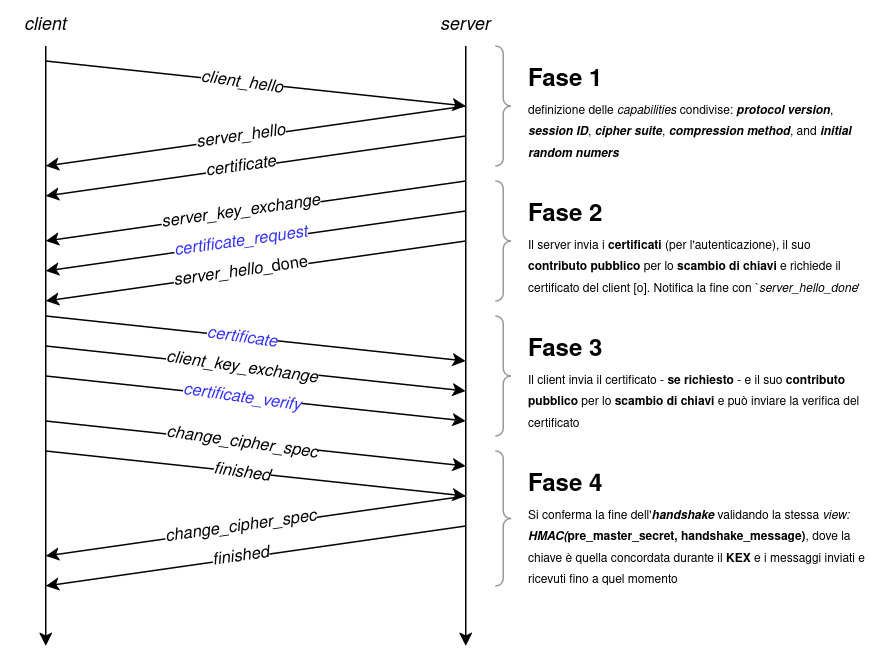
\includegraphics[width=\textwidth]{img/tls_handshake.png}
    \end{figure}

    La chiave simmetrica scambiata viene definita come \textbf{\textit{pre-master key}}, che verrà utilizzata come \textit{input} per una \textbf{KDF} - viene definita dalla versione di TLS - dalla quale verranno calcolate tre chiavi diverse.
    \begin{itemize}[nosep]
        \item \textbf{due chiavi} per l'\textbf{autenticità} (una per ogni direzione).
        \item \textbf{una chiave} per la \textbf{confidenzialità}
        \item la \textit{hash function} riferita nella \textit{cipher suite} è utilizzata in questa fase.
    \end{itemize}

    Nella \textbf{fase 4} è presente un messaggio in cui viene autenticato tutto il traffico compiuto durante l'\textit{handshake}, possiamo vederlo com un \textit{tag} di un \textbf{HMAC} calcolato utilizzado la \textbf{\textit{pre-master key}} (o meglio una chiave derivata da essa) come chiave e tutti i messaggi dell'\textit{handshake} come data.

    {\centering
        $t = \text{MAC}(\mathbf{pre\_master\_secret}, \; \mathbf{handshake\_msg})$
    \par}

    Lo scopo è identificare ``\textbf{deviazioni}'' dall'\textit{handshake} del protocollo soprattuto nella decisione del \textit{shared secret}. 

    \smallskip

    \textcolor{red}{\textbf{\textit{Ephemeral Keys}}}: nei moderni protocolli sicuri di comunicazione, le parti hanno \textbf{\textit{long-term static keys}} solamente per la fase di autenticità, le quali vengono incluse all'interno dei certificati - opzionali per i client. Queste chiavi non vengono utilizzate per garantire \textbf{confidenzialità} se vogliamo anche garantire \textbf{\textit{perfect forward security}}, infatti la compromissione di una chiave non compromette messaggi cifrati ``nel passato''.  \\
    La \textbf{confidenzialità} nel \textbf{KEX} è garantita dalle \textbf{chiave effimere} generate \textit{runtime} durante lo scambio di chiavi - \textit{ephemeral} \textbf{DH} $\rightarrow$ \textbf{DHE}, se basate su curve ellittiche: \textbf{ECDHE}. Le chiavi possono essere anche \textbf{ruotate} dopo un certo evento, ad esempio il superamento di una \textit{threshold} di dati cifrati o dopo una \textit{session resumption}.
    
    \textbf{Note}: non confondersi \textit{ephemeral keys} (che sono \textbf{asimmetriche}) con la \textbf{chiave simmetrica} che viene sempre ricalcolata, il suo riutilizzo può portare gravi vulnerabilità (ad esempio il \textit{nonce reuse}).
    \begin{itemize}[nosep]
        \item \textbf{\textit{Session ID}}: per evitare il costo di un \textbf{KEX} durante l'handshake, si può riutilizzare una sessione precedente tramite il meccanismo del \textbf{Session ID}. In questo caso, il client include nel messaggio \textit{client\_hello} un \textbf{\textit{Session ID}} relativo a una connessione passata. Se il server riconosce quell'ID, risponde con lo stesso \textbf{\textit{Session ID}}, indicando che la chiave simmetrica può essere riutilizzata. Il client, a sua volta, può accettare o rifiutare. Se accetta, la connessione viene ripristinata rapidamente senza eseguire di nuovo il protocollo di key exchange - \textit{session resumption}.
        \item \textbf{\textit{Cipher Suites}}: permette al client e al server di accordarsi su una lista comune di protocolli di sicurezza tra quelli supportati, normalmente il client propone e il server ne sceglie uno - se supportato - o nega la connessione.
        \item nella versione 1.2 di \textbf{TLS} veniva utilizzata un \textbf{\textit{RSA-baased KEX}} dove la chiave veniva decisa dal client e cifrata con la chiave pubblica del server, che non è effimera. La chiave segreta utilizzata nel \textit{RSA-based KEX} non è effimera - è stata deprecata nella versione 1.3.
    \end{itemize}

    \newpage

    \textcolor{red}{\textbf{\textit{TLS 1.3 vs. TLS 1.2}}} \\
    Nell'ultima versione di \textbf{TLS} semplifica alcune procedure durante l'\textit{handshake} e riporta il numero di scambia 3, in modo che sia retrocompatibile con il \textbf{TCP} non sicuro. Nel \textit{client\_hello} viene già inviato il contributo pubblico per uno \textbf{KEX \textit{DH-based}}. Sono state rimossi ``vecchi'' - deprecati - protocolli che poteva permettere \textbf{\textit{dowgrade attack}} a causa di configurazioni di parametri errata. Sono stati inoltre rimossi i \textit{anauthenticated cipher}. I due maggiori cambiamenti sono:
    \begin{itemize}[nosep]
        \item non è più supportato \textbf{\textit{RSA-based KEX}}
        \item aggiunto supporto per \textbf{\textit{0-RTT request}} sulle \textit{cached session} senza \textbf{\textit{replay attack protection}}
    \end{itemize}

    \medskip

    \textcolor{red}{\textbf{\textit{Downgrade Attack}}} \\
    Il \textbf{\textit{downgrade attack}} è un attacco in cui un attaccante forza client e server a usare una versione più vecchia e meno sicura di \textbf{TLS}, o cifrature deboli. Per evitarlo, \textbf{TLS} include nel messaggio \textit{fnished} dell'\textit{handshake} un \textbf{MAC} calcolato su tutti i messaggi precedenti dello scambio. Questo garantisce l'integrità dell'\textit{handshake}: se un attaccante ha manipolato i messaggi per effettuare un \textit{downgrade}, il MAC nel messaggio \textit{fnished} non sarà valido e la connessione verrà interrotta.
\end{flushleft}

\section{Other Secure Communication Protocol}

\begin{flushleft}
    \textcolor{red}{\textbf{\textit{Secure Messaging}}}: si riferisce a quei protocolli basati su comunicazioni asincrone. In genere, è necessario supportare ``gruppi'', possibili destinatari non raggiungibili (\textit{offline}) e altri possibili requisiti. Protocolli popolari:
    \begin{itemize}[nosep]
        \item \textbf{\textit{Signal Protocol}}: formalmente denominati - basati - su protocolli \textbf{\textit{Off-the-Record (OTR)}} e protocolli di \textbf{\textit{TextSecure}}, utilizzati da \textit{whatsapp} e altri.
        \item \textbf{\textit{Message Layer Security - MLS}}: è un protocollo in via di standardizzazione per la messaggistica di gruppo, potrebbe essere utile per l'\textbf{IoT} e altri scenari - ad esempio per la comunicazione \textit{publisher/subscriber}.
    \end{itemize}

    Comunicazioni crittografate \textit{end-to-end} rappresentano un coltello a doppio taglio nel contesto della sicurezza. Possono garantire \textbf{\textbf{privacy}} e \textit{cyber-security} agli utenti, ma al contempo possono rendere più difficile per le \textbf{agenzia delle forze dell'ordine} per intercettare comunicazioni illecite - terroristi, ecc.
    \begin{itemize}[nosep]
        \item ad esempio il caso storico di \textbf{PGP}.
    \end{itemize}
    Attualmente non c'è una soluzione chiara per riuscire ad intercettare traffico cifrato illecito.

    \medskip

    \textcolor{red}{\textbf{\textit{Secure Web Conferencing}}}: l'idea è quella di garantire crittografia \textit{end-to-end} nelle comunicazioni audio e video \textit{real-time}, quali sono le sfide:
    \begin{itemize}[nosep]
        \item valutazione delle \textit{performance} dei protocolli crittografici (sia \textit{server-side} che \textit{client-side})
        \item requisiti peculiari - registrare chiamate \textit{server-side} cifrate.
        \item paradossi - come ottenere didascalie se le chiamate sono cifrate.
    \end{itemize}

\end{flushleft}

\section{HTTPs}

\begin{flushleft}

    \textcolor{red}{\textbf{\textit{HTTPs} e \textit{Virtual Hosting}}} \\

    \begin{figure}[h]
        \centering
        \begin{minipage}[t]{0.45\textwidth}
            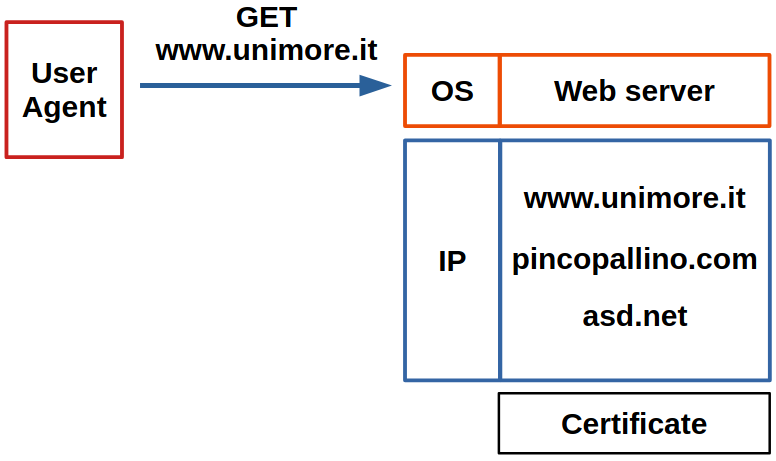
\includegraphics[width=\textwidth]{img/https_vh_1.png}
            \caption{Architettura monolita}
        \end{minipage}
        \hfill
        \begin{minipage}[t]{0.45\textwidth}
            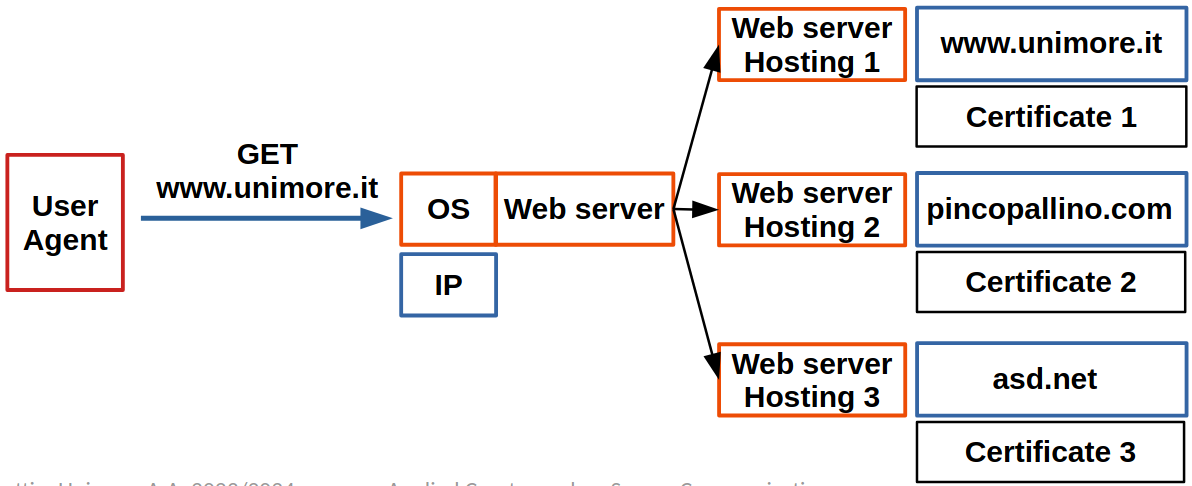
\includegraphics[width=\textwidth]{img/https_vh_2.png}
            \caption{Architettura distribuita}
        \end{minipage}
    \end{figure}

    Il \textit{virtual hosting} permette di gestire più \textit{web application} sullo stesso \textit{web server}. Nel caso di architettura \textbf{distribuita} ogni macchina può utilizzare un certificato differente, per evitare che il nome del \textit{web server} venga inviato cifrato nel \textit{payload} del messaggio, viene utilizzato un campo nel \textit{client\_hello} - presente tramite una sua estensione - dell'\textit{TLS handshake} chiamato \textbf{\textit{Server Name Indicator}} che permette di comunicare in chiaro, il \textit{server web} di destinazione.
    \begin{itemize}[nosep]
        \item \textbf{\textit{Encrypted Server Name Indicator - ESNI}}: è un'estensione del protocollo \textbf{TLS} che protegge la privacy dell'utente cifrando il anche \textbf{SNI} indicato durante l'\textit{handshake}.
        \item \textbf{\textit{Encrypted Client Hello - ECH}}: è una versione evoluta
    \end{itemize}
    
    \medskip

    \textcolor{red}{\textbf{\textit{SSL Stripping to HTTPs}}} \\
    Se un client cerca di accedere ad una \textit{web app} tramite la sua interfaccia non sicura - \textbf{porta 80} - la \textit{best practice} per il \textit{web server} è quella di fare un \textit{REDIRECT} all'\textit{endpoint} sicuro. \\
    L'\textbf{\textit{SSL Stripping}} è il nome che si da ad una tecnica di attacco \textbf{MitM} che coinvelge la capacità di \textbf{riscrivere l'\textit{header} HTTP} e il contenuto dell'\textbf{HTML} per rimuovere qualunque possibile \textbf{ridirezione} al servizio \textbf{HTTPs}.
    \begin{itemize}[nosep]
        \item \textbf{\textit{HTTP String Transport Security - HSTS}}: il server imposta \textbf{\textit{Strict-Transport-Security}} nella prima richiesta del client per dirgli di usare sempre HTTPs dalla richiesta successiva. È comunque possibile per un attaccante riscrivere l'\textbf{URi} in modo tale che le \textit{security policy} definite nell'\textbf{HSTS} non vengano applicate.
    
        {\centering
            \texttt{www.unimore.it} $\rightarrow$ \texttt{wwww.unimore.it}
        \par}

        \item configurare il client per utilizzare sempre connessioni \textbf{HTTPs}
    \end{itemize}
\end{flushleft}